\section{Inledning}
Systemet kommer bestå av en robot som i sig består av tre undermoduler. Utöver detta tillkommer mjukvara på roboten och PC som används för manuell styrning och övervakning. Detta är en systemskiss som ska ge en grov översikt hur systemet ska implementeras. Detta ska sedan vara underlag för designspecifikationen. 
\newline
\newline
Varje enskild modul kommer att ha en egen processor och dessa kommer sedan kommunicera över en bus. Systemet kommer kommunicera med en PC över blåtand. När systemet är klart för leverans ska det kunna följa en bana som visas nedan och plocka upp och sätta ned paket på de utsatta stationerna B och C. 

\centerline{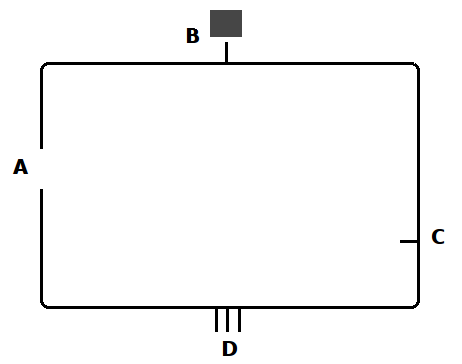
\includegraphics[scale=0.4]{figur}}